\subsection{Kori\v s\' cenje onlajn sistema Nacionalne slu\v zbe}

Onlajn sistem Nacionalne slu\v zbe je veb aplikacija koja omogu\' cava obavljanje odre\dj enih poslovnih funkcija vezanih za eksterne korisnike putem interneta. Kori\v s\' cenjem onlajn sistema, eksterni korisnici mogu uz manje napora i br\v ze da dobiju usluge Nacionalne slu\v zbe.\\

Onlajn sistem prepoznaje dve vrste eksternih korisnika: \textit{nezaposleno lice}, i \textit{predstavnik kompanije sa kojom Nacionalna slu\v zba sara\dj uje} (radi jednostavnosti, ovaj subjekat \'cemo nazivati \textit{kompanija}), i jedan tip internog korisnika: \textit{savetnik za poslodavce}. Na Slici \ref{dsu: koriscenje onlajn sistema nacionalne sluzbe} prikazani su navedeni korisnici i procesi u kojima u\v cestvuju, a koje \'cemo opisati u daljem tekstu.\\

Za oba korisnika je omogu\' ceno pravljenje naloga i prijavljivanje na sistem. Pravljenje naloga za nezaposlena lica i kompanije je u osnovi sli\v cno. Razlike izme\dj u ova dva procesa su: dodatne aktivnosti koje Nacionalna slu\v zba mora da preuzme pri otvaranju naloga za kompanije i informacije od zna\v caja (formular u korisni\v ckom interfejsu). Zbog toga \' cemo prvo opisati Pravljenje naloga (slu\v caj upotrebe \ref{su: pravljenje naloga}), a zatim opisati pojedinosti pravljenja naloga za kompanije, \v sto podrazumeva Odobrenje naloga za kompanije (slu\v caj upotrebe \ref{su: odobrenje naloga za kompanije}). Slu\v cajem upotrebe \ref{su: prijavljivanje na sistem} detaljno je opisan proces prijavljivanja na sistem. Na kraju prikazujemo procese Pretraga oglasa poslova (slu\v caj upotrebe \ref{su: pretraga oglasa poslova}) i Otvaranje oglasa za novu ponudu za posao (slu\v caj upotrebe \ref{su: otvaranje oglasa za novu ponudu za posao}). Za svaki opisan proces dajemo i izgled korisni\v ckog interfejsa.

\begin{figure}[H]
	\centering
	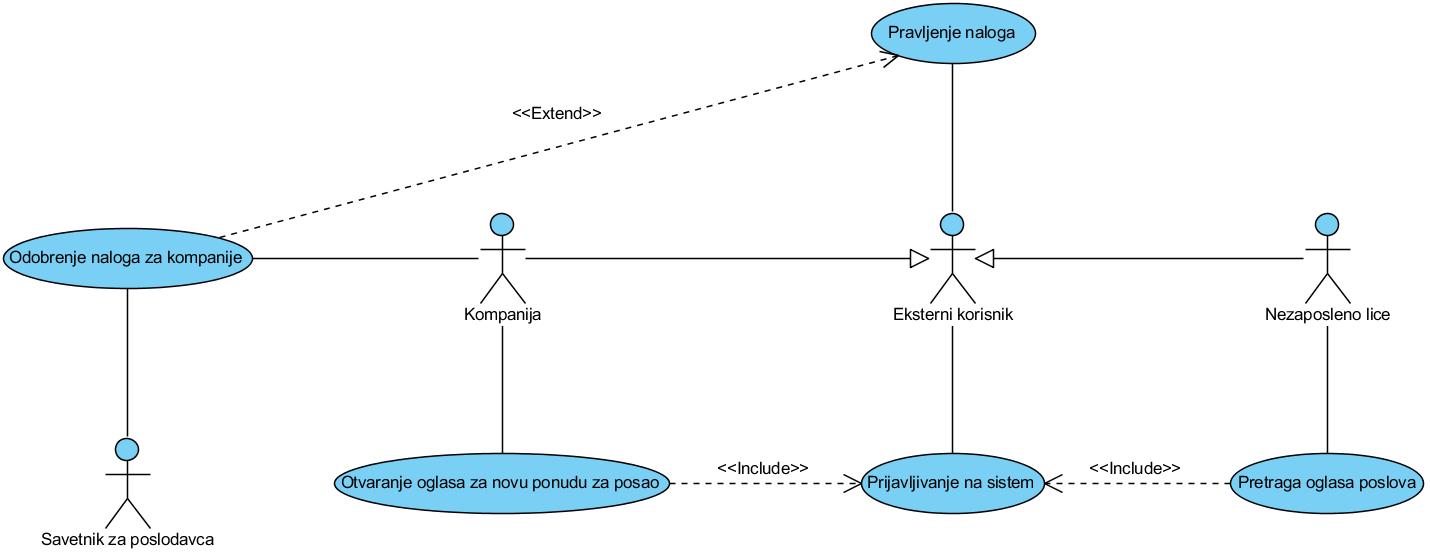
\includegraphics[width=\textwidth]{dijagrami/dijagrami-slucajeva-upotrebe/onlajn-sistem.png}
	\caption{Dijagram slu\v cajeva upotrebe procesa ''Kori\v s\' cenje onlajn sistema Nacionalne slu\v zbe''.}
	\label{dsu: koriscenje onlajn sistema nacionalne sluzbe}
\end{figure}

\subsubsection{Slu\v caj upotrebe: Pravljenje naloga}
\label{su: pravljenje naloga}

\noindent U\v cesnici: Eksterni korisnik (u daljem tekstu EK)
\\
\\ Preduslovi: Ako je tip EK ''Nezaposleno lice'', onda EK ima evidentacioni karton.
\\
\\ Postuslovi: Ili je EK uspe\v sno napravio nalog ili je stanje ostalo nepromenjeno.
\\ 
\\ Glavni tok:
\begin{enumerate}
	\item EK pristupa onlajn sistemu Nacionalne slu\v zbe.
	\item Sistem prikazuje po\v cetnu stranu \ref{for: index}.
	\item EK bira opciju ''Registracija novog korisnika''.
	\item U zavisnosti od tipa EK, Sistem prikazuje odgovaraju\' ci formular.
	\item EK popunjava formular.
	\item EK bira opciju ''Sa\v cuvaj i nastavi''.
	\item Sistem, na osnovu unetih podataka, proverava da li ve\'c postoji takav korisnik.
	\item Sistem ustanovljava da postoji takav korisnik.
	\begin{enumerate}
		\item Sistem prikazuje poruku sa obave\v stenjem i nudi EK opciju da promeni \v lozinku (ukoliko ju je zaboravio).
		\item EK bira da li \v zeli da promeni lozinku.
		\item EK bira da promeni lozinku.
		\begin{enumerate}
			\item Sistem tra\v zi od EK da unese email adresu.
			\item NK unosi email adresu i potvr\dj uje unos.
			\item Sistem obave\v stava EK da mu je poslata nova lozinka na email adresu.
			\item Slu\v caj upotrebe se zavr\v sava.
		\end{enumerate}
		\item EK bira da ne promeni lozinku, pa se prelazi na korak 2.
	\end{enumerate}
	\item Sistem ustanovljava da ne postoji takav korisnik, pa se prelazi na korak 10.
	\item Sistem utvr\dj uje tip EK.
	\item Sistem je utvrdio da je tip EK ''Nezaposleno lice'', pa se prelazi na korak 13.
	\item Sistem je utvrdio da je tip EK ''Kompanija''.
	\begin{enumerate}
		\item Prelazi se na slu\v caj upotrebe \ref{su: odobrenje naloga za kompanije}.
		\item Po zavr\v setku slu\v caja upotrebe, sistem obave\v stava EK da \' ce mu odgovor sti\' ci na email.
		\item Slu\v caj upotrebe se zavr\v sava.
	\end{enumerate}
	\item Sistem otvara novi nalog sa unetim podacima, a zatim \v salje poruku na unetu email adresu za potvr\dj ivanje.
	\item Sistem obave\v stava EK da je nalog uspe\v sno otvoren i da treba da potvrdi otvaranje naloga na email-u.
	\item Kada EK potvrdi otvaranje naloga na email-u, sistem mu prikazuje obave\v stenje da je otvaranje naloga kompletirano.
\end{enumerate}

\noindent Alternativni tokovi: 
\begin{description}
	\item[A1. Nedostupnost sistema] ~\\
	Ukoliko u bilo kom od koraka 1--4 Glavnog toka ne do\dj e do prikaza korisni\v ckog interfejsa (na primer, zbog sporog interneta), EK mo\v ze da sa\v ceka, pa da poku\v sa ponovo, ili da odustane od pravljenja naloga.
	
	\item[A2. Neispravnost unetih podataka] ~\\
	Ukoliko u koraku 6 Glavnog toka sistem utvrdi da neki podatak nije validan ili neko obavezno polje nije popunjeno, sistem generi\v se poruku o gre\v sci i zahteva od EK da ispravno popuni formu. Izvr\v savanje se nastavlja u koraku 5 Glavnog toka.
\end{description}

\subsubsection{Slu\v caj upotrebe: Odobrenje naloga za kompanije}
\label{su: odobrenje naloga za kompanije}

\noindent U\v cesnici: Kompanija (u daljem tekstu K), Savetnik za poslodavce (u daljem tekstu SP)
\\
\\ Preduslovi: SP ima pristup sistemu i autorizovan je. K ima li\v cnu kartu. Dostupne su informacije iz formulara \ref{for: k-registracija}.
\\
\\ Postuslovi: Ili je K uspe\v sno odobreno pravljenje naloga ili je zabele\v zen poziv za saradnju ili je stanje ostalo nepromenjeno i izdata je poruka o gre\v sci.
\\ 
\\ Glavni tok:
\begin{enumerate}
	\item Sistem proverava da li je ostvarena saradnja izme\dj u K i Nacionalne slu\v zbe.
	\item Sistem je ustanovio da je ostvarena saradnja, pa se prelazi na korak 4.
	\item Sistem je ustanovio da nije ostvarena saradnja.
	\begin{enumerate}
		\item Sistem nudi K opciju da podnese zahtev za saradnju.
		\item K bira da podnese zahtev za saradnju.
		\begin{enumerate}
			\item Sistem tra\v zi od K da unese broj li\v cne karte.
			\item K unosi broj li\v cne karte.
			\item Sistem automatski pronalazi SP koji \' ce biti zadu\v zen za K.
			\item Sistem bele\v zi novog poslodavca (na osnovu podataka iz formulara) i zadu\v zuje prona\dj enog SP za K.
			\item Prelazi se na korak 4.
		\end{enumerate}
		\item K bira da ne podnese zahtev sa saradnju, pa se slu\v caj upotrebe zavr\v sava. Ukoliko je slu\v caj upotrebe pokrenut iz slu\v caja upotrebe ''Pravljenje naloga'', onda se i taj slu\v caj upotrebe zavr\v sava.
	\end{enumerate}
	\item Sistem pronalazi SP koji je zadu\v zen za K.
	\item Sistem \v salje novi zahtev SP za autorizacijom novog naloga.
	\item SP proverava da li je zahtev u skladu sa protokolom.
	\item SP ustanovljava da zahtev jeste u skladu sa protokolom.
	\begin{enumerate}
		\item SP autorizuje zahtev.
		\item Prelazi se na korak 9.
	\end{enumerate}
	\item SP ustanovljava da zahtev nije u skladu sa protokolom.
	\begin{enumerate}
		\item SP odbija zahtev, i popunjava polje sa obrazlo\v zenjem.
		\item Sistem generi\v se poruku koja se \v salje na unetu email adresu, a koja uklju\v cuje obave\v stenje da je zahtev odbijen i obrazlo\v zenje.
		\item Slu\v caj upotrebe se zavr\v sava.
	\end{enumerate}
	\item Sistem otvara novi nalog sa unetim podacima, a zatim \v salje poruku na unetu email adresu za potvr\dj ivanje.
	\item Kada K potvrdi otvaranje naloga na email-u, sistem joj prikazuje obave\v stenje da je otvaranje naloga kompletirano.
\end{enumerate}

\noindent Alternativni tokovi: 
\\/

\subsubsection{Slu\v caj upotrebe: Prijavljivanje na sistem}
\label{su: prijavljivanje na sistem}

\noindent U\v cesnici: Eksterni korisnik (u daljem tekstu EK)
\\
\\ Preduslovi: /
\\
\\ Postuslovi: Ili se EK uspe\v sno prijavio na sistem ili je izdata poruka o gre\v sci.
\\ 
\\ Glavni tok:
\begin{enumerate}
	\item Sistem prikazuje formular za prijavljivanje na sistem (formular \ref{for: prijava}).
	\item EK unosi korisni\v cko ime i lozinku.
	\item Sistem, na osnovu unetih podataka, proverava da li ve\'c postoji takav korisnik.
	\item Sistem ustanovljava da postoji takav korisnik.
	\begin{enumerate}
		\item Sistem proverava da li se uneta lozinka poklapa sa lozinkom u bazi sistema.
		\item Sistem ustanovljava da se uneta lozinka poklapa, pa se slu\v caj upotrebe zavr\v sava.
		\item Sistem ustanovljava da se lozinka ne poklapa.
		\begin{enumerate}
			\item Sistem prikazuje poruku sa obave\v stenjem i nudi EK opciju da promeni \v lozinku (ukoliko ju je zaboravio).
			\item EK bira da li \v zeli da promeni lozinku.
			\item EK bira da promeni lozinku.
			\begin{enumerate}
				\item Sistem tra\v zi od EK da unese email adresu.
				\item NK unosi email adresu i potvr\dj uje unos.
				\item Sistem obave\v stava EK da mu je poslata nova lozinka na email adresu.
				\item Slu\v caj upotrebe se zavr\v sava.
			\end{enumerate}
			\item EK bira da ne promeni lozinku, pa se prelazi na korak 1.
		\end{enumerate}
	\end{enumerate}
	\item Sistem ustanovljava da ne postoji takav korisnik.
	\begin{enumerate}
		\item Sistem obave\v stava EK da ne postoji korisnik sa unetim korisni\v ckim imenom.
		\item EK bira da poku\v sa ponovo, pa se prelazi na korak 1.
	\end{enumerate}
\end{enumerate}

\noindent Alternativni tokovi: 
\begin{description}
	\item[A1. Odustajanje od prijavljivanja] ~\\
		Ukoliko u bilo kom koraku Glavnog toka EK odlu\v ci da odustane od prijavljivanja na sistem i slu\v caj upotrebe je pokrenut iz nekog drugog slu\v caja upotrebe, sistem generi\v se gre\v sku. Slu\v caj upotrebe se nasilno zavr\v sava.
\end{description}

\subsubsection{Slu\v caj upotrebe: Pretraga oglasa poslova}
\label{su: pretraga oglasa poslova}

\noindent U\v cesnici: Nezaposleno lice (u daljem tekstu NL)
\\
\\ Preduslovi: /
\\
\\ Postuslovi: NL je, potencijalno, poslao ponudu za razgovor za posao nekoj kompaniji, ili vi\v se njih. Ako jeste, onda su kompanijama automatski podneti zahtevi.
\\ 
\\ Glavni tok:
\begin{enumerate}
	\item NL bira da se prijavi na sistem.
	\item Prelazi se na slu\v caj upotrebe \ref{su: prijavljivanje na sistem}.
	\begin{enumerate}
		\item U slu\v caju uspe\v snog zavr\v savanja, prelazi se na korak 3.
		\item Ina\v ce, izdaje se poruka o gre\v sci i slu\v caj upotrebe se zavr\v sava.
	\end{enumerate}
	\item Sistem prikazuje listu oglasa za posao koji postoje u bazi sistema.
	\item NL bira jedan posao.
	\item Sistem prikazuje detaljne informacije o oglasu za posao.
	\item NL bira da li \v zeli da kontaktira kompaniju.
	\item NL bira da kontaktira kompaniju.
	\begin{enumerate}
		\item NL popunjava formular za kontaktiranje kompanije (formular \ref{for: fl-slanjePonude}).
		\item NL \v salje formular.
		\item Sistem automatski dopunjava popunjeni formular informacijama o NL iz baze sistema.
		\item Sistem \v salje zahtev za razgovor za posao kompaniji, pa se prelazi na korak 3.
	\end{enumerate}
	\item NL bira da ne kontaktira kompaniju, pa se prelazi na korak 9.
	\item NL bira da se vrati na listu oglasa za posao.
	\item Koraci 3--9 se ponavljaju dok NL ne zavr\v si sa pretragom oglasa za poslove.
	\item NL se odjavljuje sa sistema.
\end{enumerate}

\noindent Alternativni tokovi: 
\begin{description}
	\item[A1. Promena liste oglasa] ~\\
		U bilo kom koraku Glavnog toka EK mo\v ze da podesi da mu se prikazuju poslovi odre\dj ene kategorije, u odre\dj enom gradu, i sli\v cno. Prilikom svakog odabira, sistem izdvaja iz baze samo one poslove koje zadovoljavaju uslove koje se odabrao EK. Izvr\v savanje se nastavlja u koraku 3.
\end{description}

\subsubsection{Slu\v caj upotrebe: Otvaranje oglasa za novu ponudu za posao}
\label{su: otvaranje oglasa za novu ponudu za posao}

\noindent U\v cesnici: Kompanija (u daljem tekstu K)
\\
\\ Preduslovi: /
\\
\\ Postuslovi: K je objavio oglas posao.
\\ 
\\ Glavni tok:
\begin{enumerate}
	\item K bira da se prijavi na sistem.
	\item Prelazi se na slu\v caj upotrebe \ref{su: prijavljivanje na sistem}.
	\begin{enumerate}
		\item U slu\v caju uspe\v snog zavr\v savanja, prelazi se na korak 3.
		\item Ina\v ce, izdaje se poruka o gre\v sci i slu\v caj upotrebe se zavr\v sava.
	\end{enumerate}
	\item K bira da objavi oglas za posao.
	\item Sistem tra\v zi od K da navede detalje o radnom mestu.
	\item K navodi detalje o radnom mestu.
	\item Sistem tra\v zi od K da popuni formular o konkursu na radno mesto (formular \ref{for: k-noviOglas}).
	\item K popunjava formular, a zatim potvr\dj uje izbor.
	\item Sistem registruje novi oglas u bazi.
	\item K se odjavljuje sa sistema.
\end{enumerate}

\noindent Alternativni tokovi: 
\\/

\subsubsection{Dijagrami sekvence}

\begin{figure}[H]
	\centering
	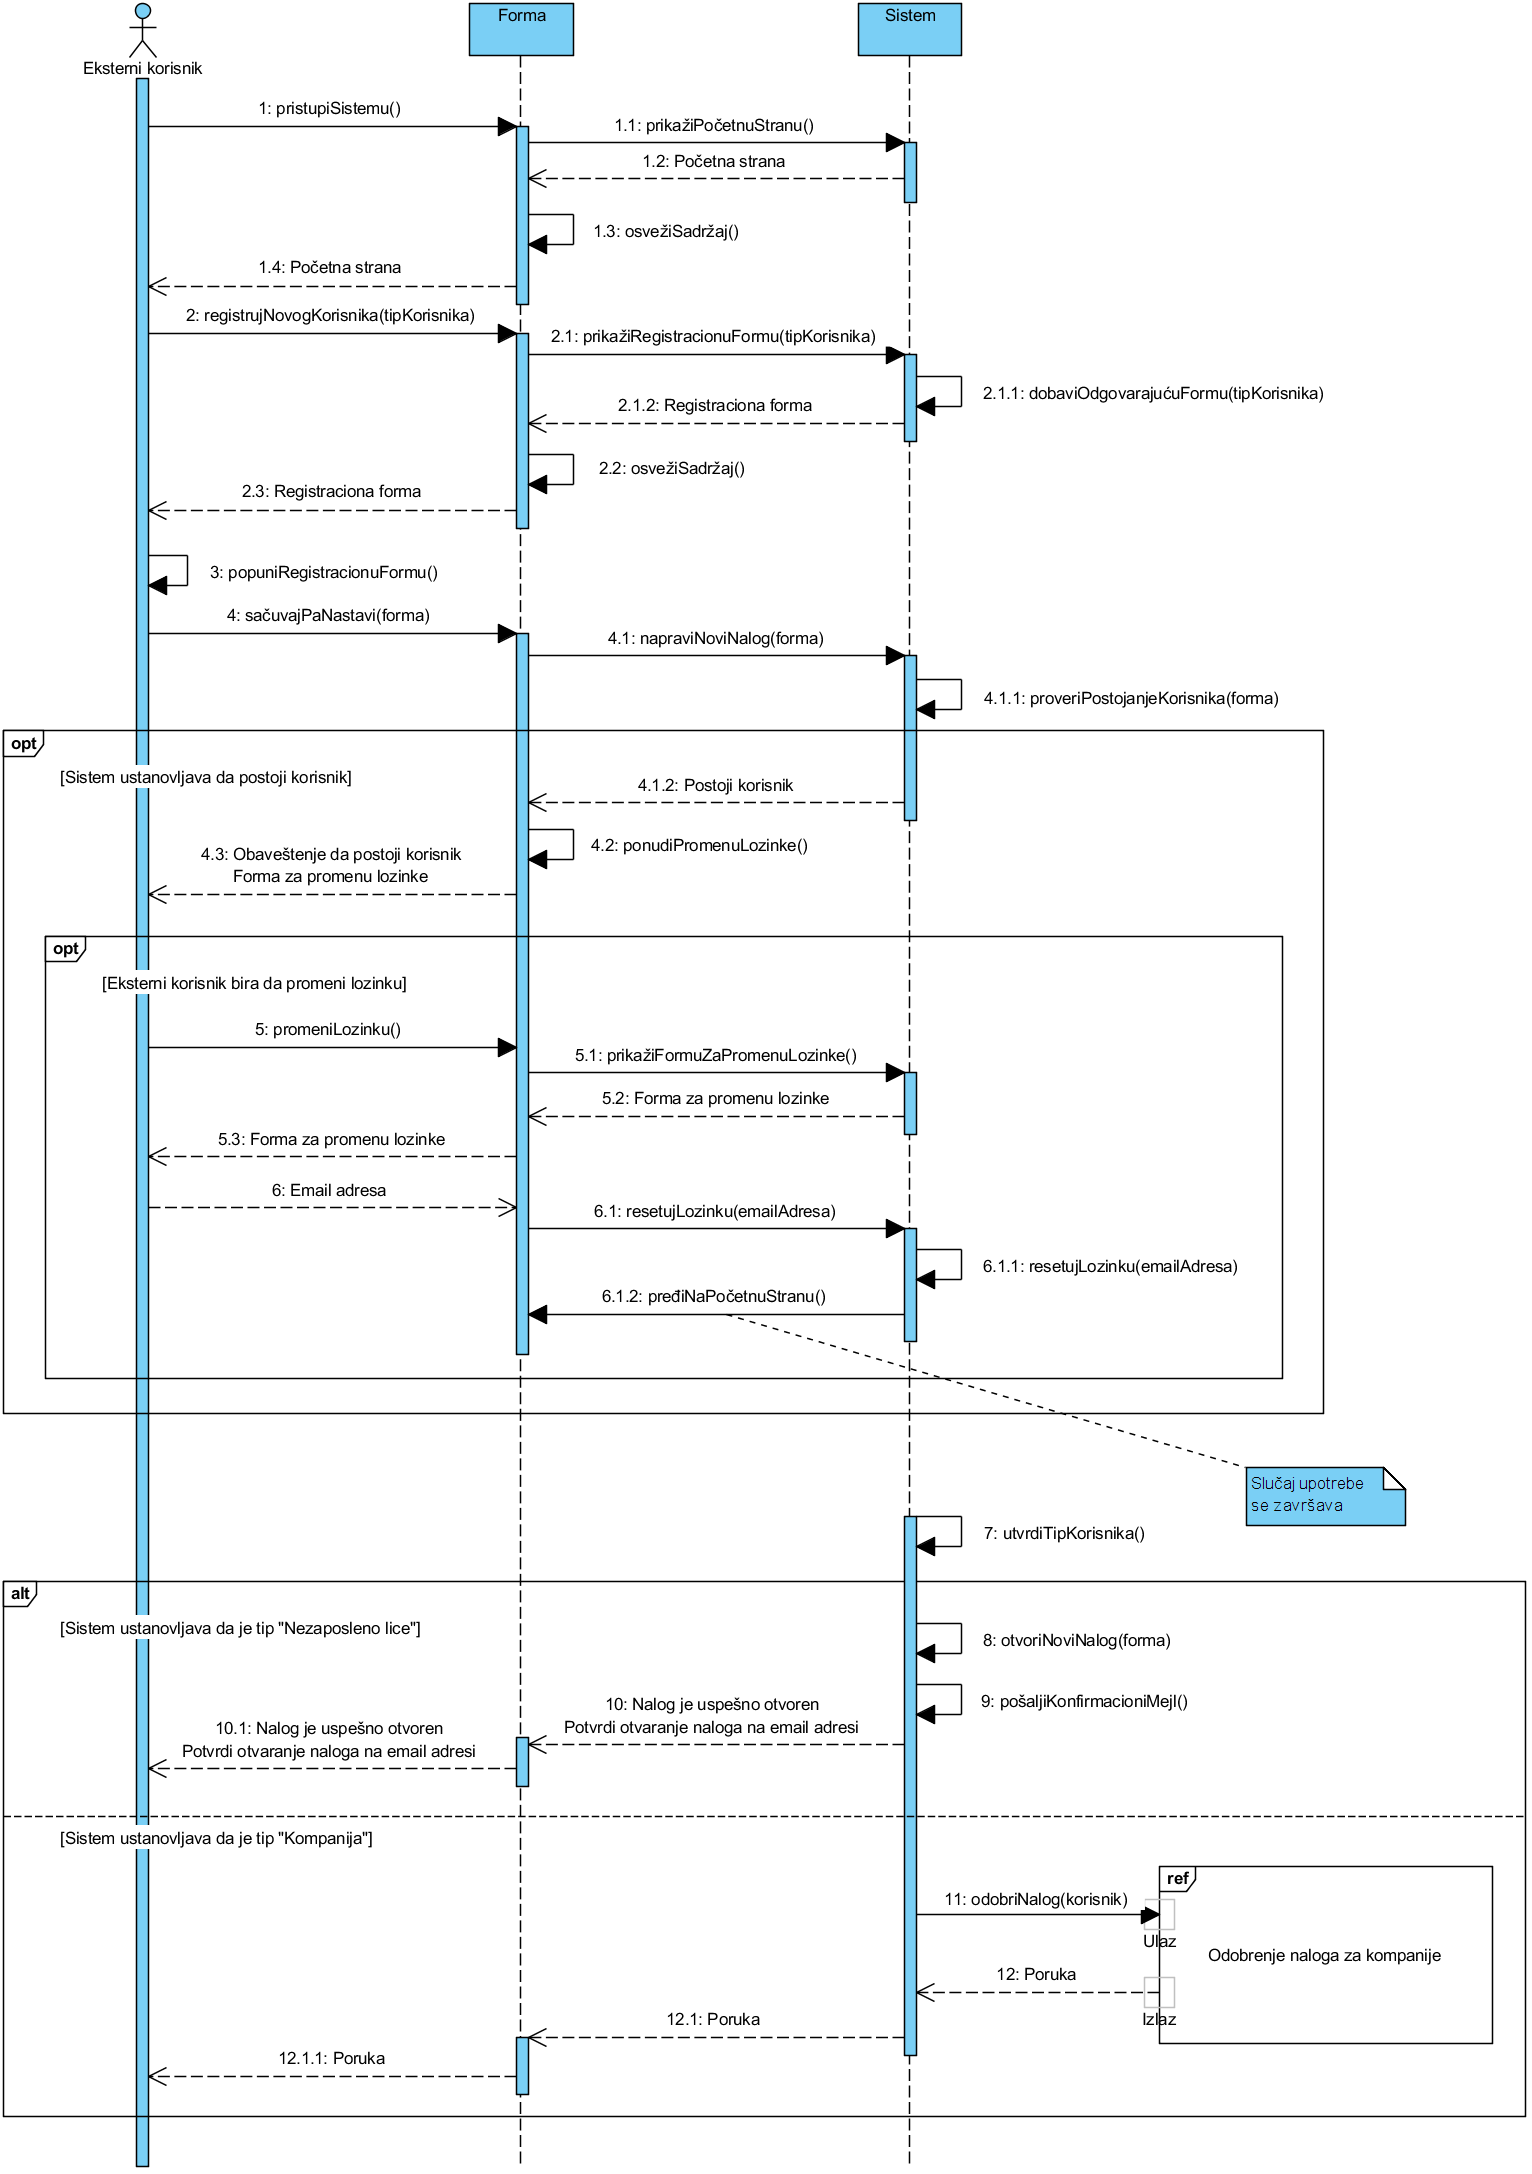
\includegraphics[width=0.87\textwidth]{dijagrami/dijagrami-sekvence/pravljenje-naloga.png}
	\caption{Dijagram sekvence slu\v caja upotrebe ''Pravljenje naloga'' (\ref{su: pravljenje naloga}).}
\end{figure}

\begin{figure}[H]
	\centering
	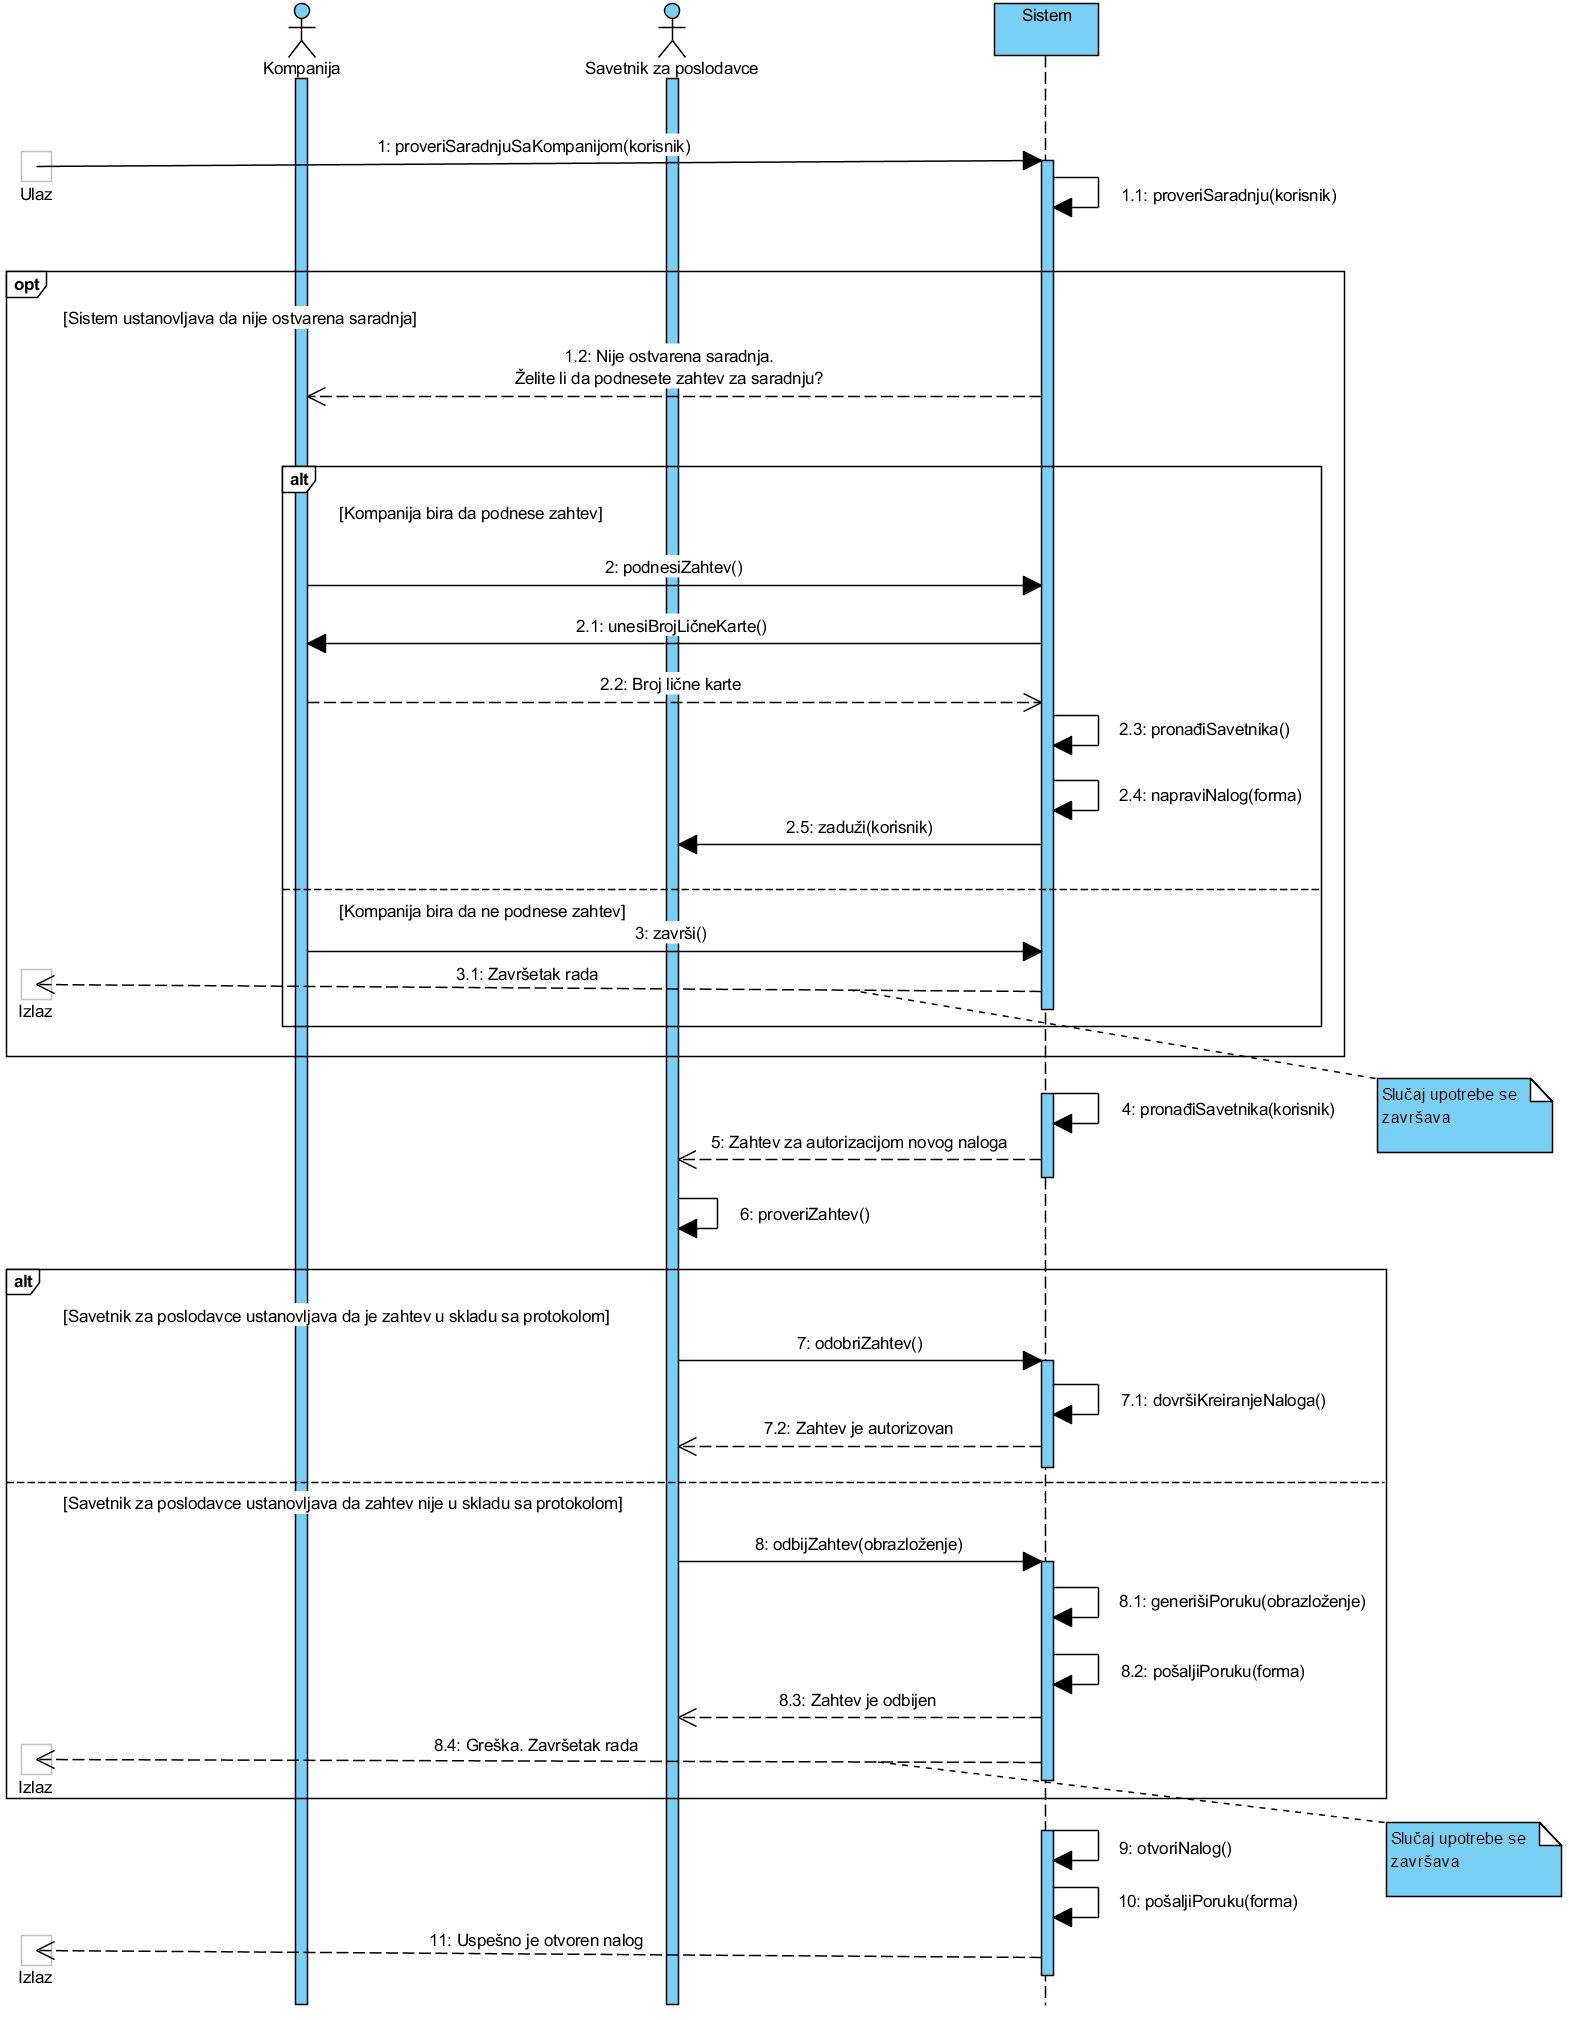
\includegraphics[width=\textwidth]{dijagrami/dijagrami-sekvence/odobrenje-naloga-za-kompanije.png}
	\caption{Dijagram sekvence slu\v caja upotrebe ''Odobrenje naloga za kompanije'' (\ref{su: odobrenje naloga za kompanije}).}
\end{figure}

\begin{figure}[H]
	\centering
	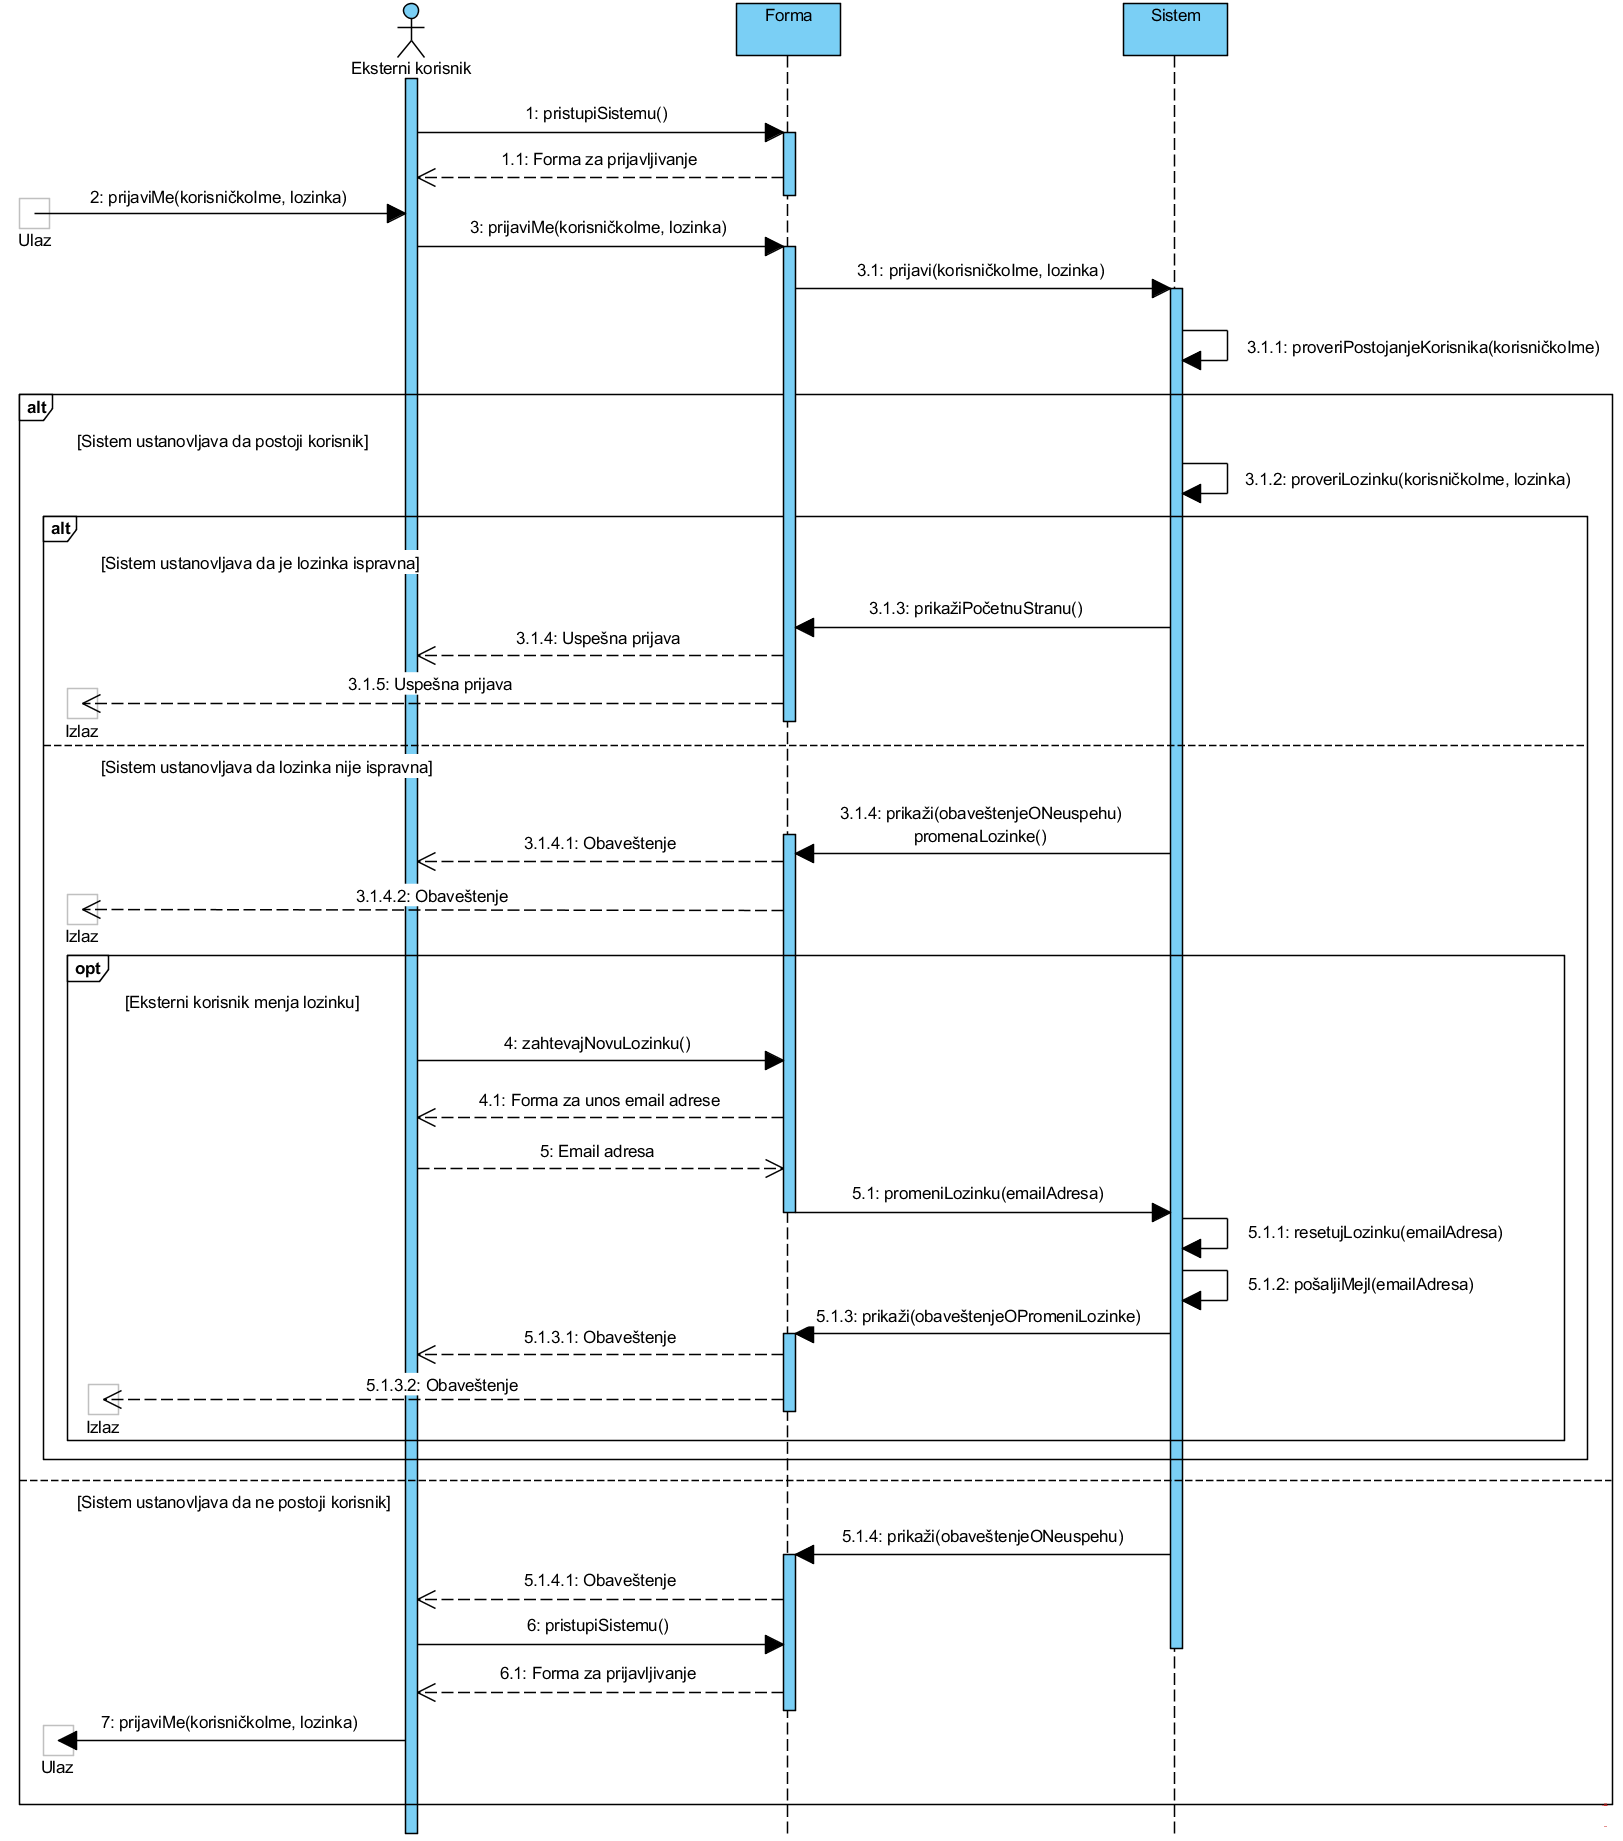
\includegraphics[width=\textwidth]{dijagrami/dijagrami-sekvence/prijavljivanje-na-sistem.png}
	\caption{Dijagram sekvence slu\v caja upotrebe ''Prijavljivanje na sistem'' (\ref{su: prijavljivanje na sistem}).}
\end{figure}

\begin{figure}[H]
	\centering
	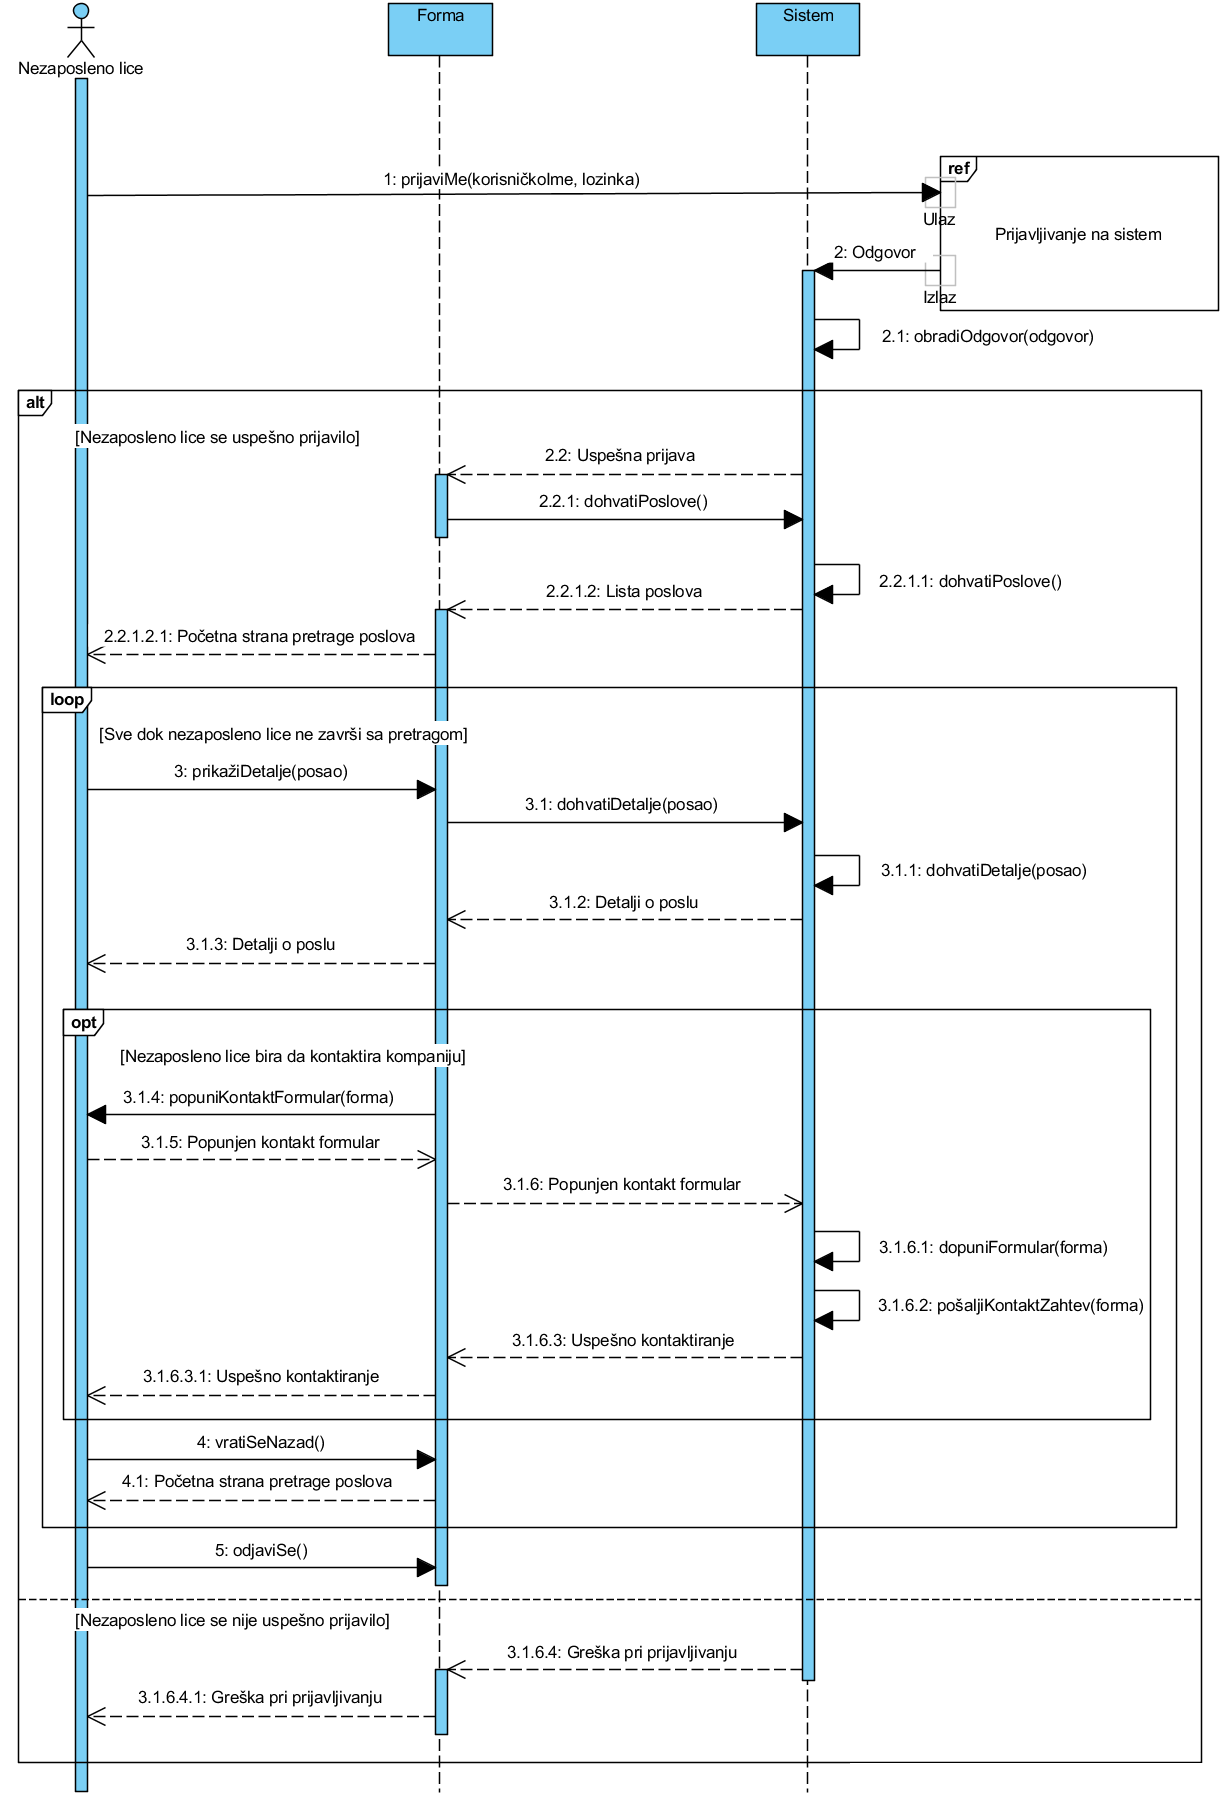
\includegraphics[width=0.9\textwidth]{dijagrami/dijagrami-sekvence/pretraga-oglasa-poslova.png}
	\caption{Dijagram sekvence slu\v caja upotrebe ''Pretraga oglasa poslova'' (\ref{su: pretraga oglasa poslova}).}
\end{figure}

\begin{figure}[H]
	\centering
	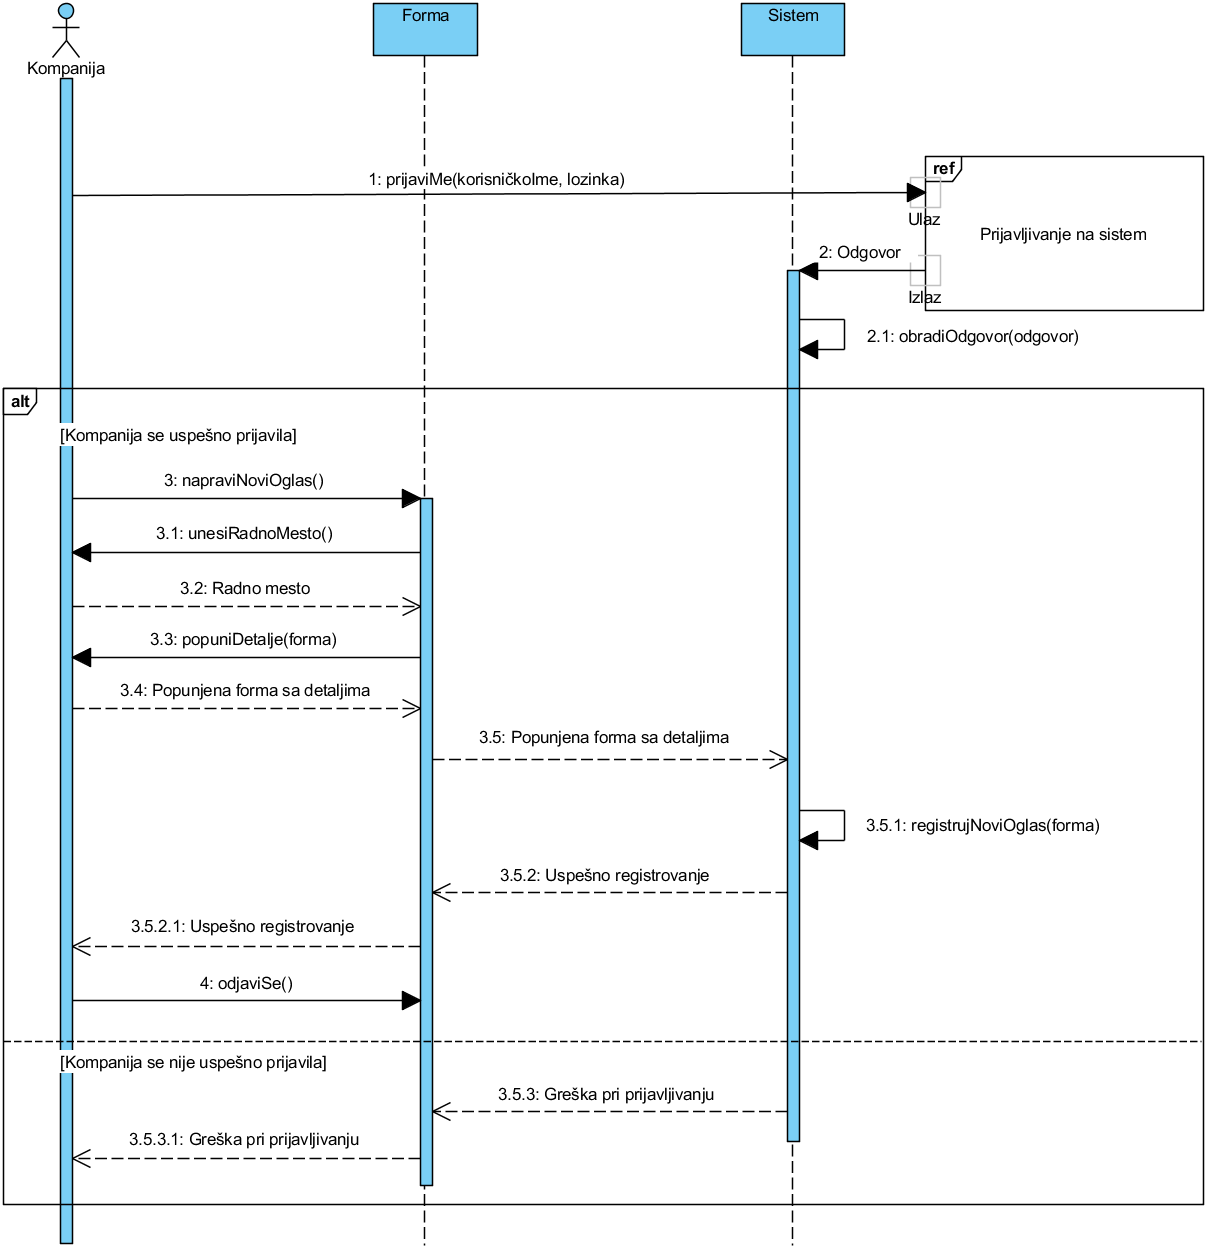
\includegraphics[width=\textwidth]{dijagrami/dijagrami-sekvence/otvaranje-oglasa-za-novu-ponudu-za-posao.png}
	\caption{Dijagram sekvence slu\v caja upotrebe ''Otvaranje oglasa za novu ponudu za posao'' (\ref{su: otvaranje oglasa za novu ponudu za posao}).}
\end{figure}

\newpage
\subsubsection{Formulari}

Prvo prikazujemo primere izgleda korisni\v ckog interfejsa za sve eksterne korisnike. Ovi formulari su vidljivi svim posetiocima onlajn sistema Nacionalne slu\v zbe.

\begin{figure}[H]
	\centering
	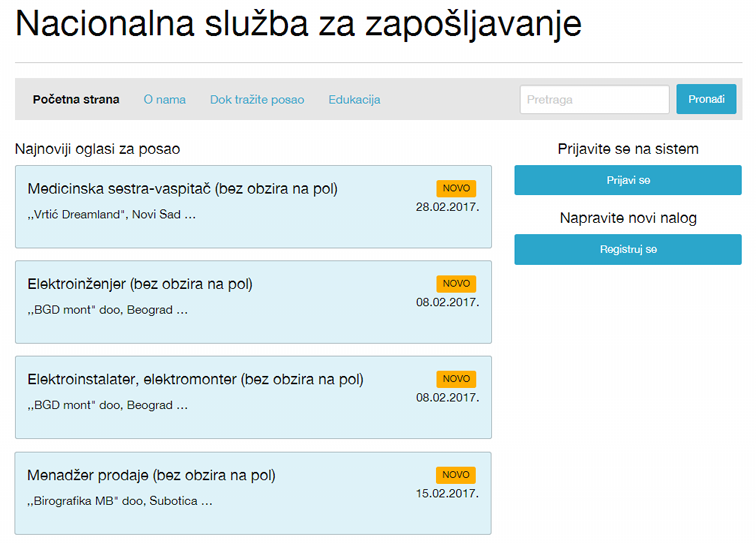
\includegraphics[width=\textwidth]{korisnicki-interfejs/slike/index.png}
	\caption{Po\v cetna strana.}
	\label{for: index}
\end{figure}

\begin{figure}[H]
	\centering
	
\includegraphics[width=\textwidth]{korisnicki-interfejs/slike/prijava.png}
	\caption{Prijavljivanje na sistem.}
	\label{for: prijava}
\end{figure}

\begin{figure}[H]
	\centering
	
\includegraphics[width=\textwidth]{korisnicki-interfejs/slike/registracija.png}
	\caption{Registracija na sistem.}
	\label{for: registracija}
\end{figure}

Formulari za registraciju na sistem se razlikuju za fizi\v cka i pravna lica. Dajemo primere oba formulara.

\begin{figure}[H]
	\centering
	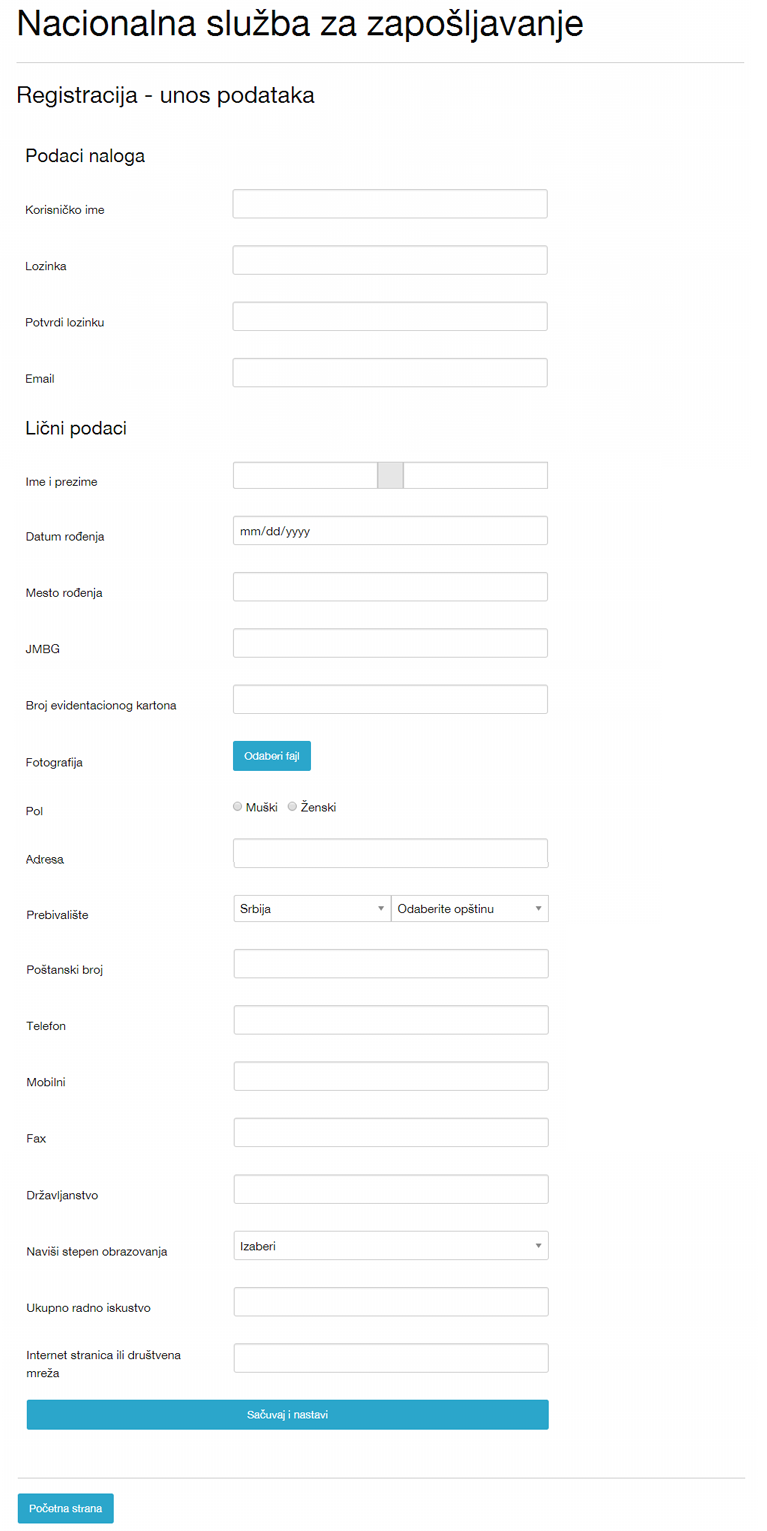
\includegraphics[height=0.95\textheight]{korisnicki-interfejs/slike/fl-registracija.png}
	\caption{Fizi\v cko lice: Registracija.}
	\label{for: fl-registracija}
\end{figure}

\begin{figure}[H]
	\centering
	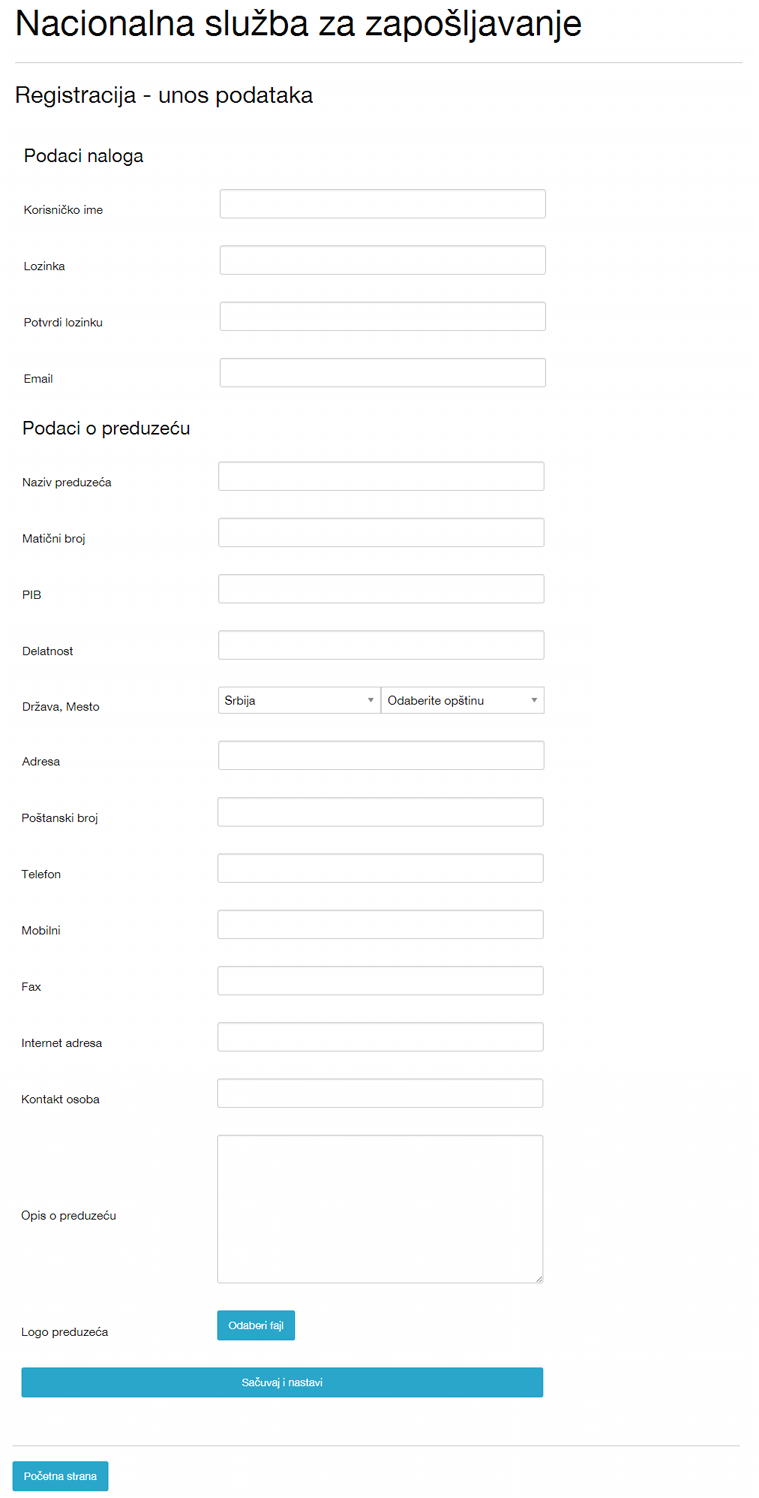
\includegraphics[height=0.95\textheight]{korisnicki-interfejs/slike/k-registracija.png}
	\caption{Kompanija: Registracija.}
	\label{for: k-registracija}
\end{figure}

Naredni formulari su vidljivi isklju\v civo fizi\v ckim licima, i to nakon uspe\v snog prijavljivanja na sistem.

\begin{figure}[H]
	\centering
	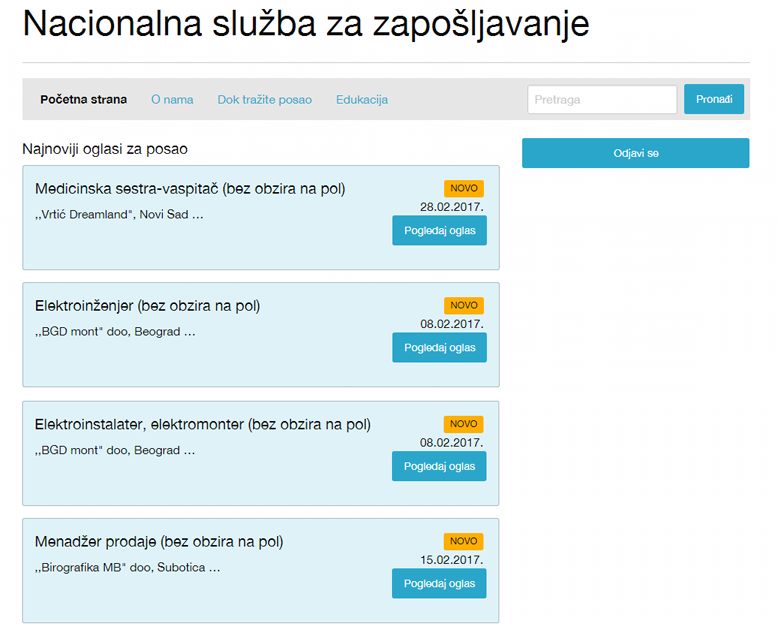
\includegraphics[width=\textwidth]{korisnicki-interfejs/slike/fl-index.png}
	\caption{Fizi\v cko lice: Po\v cetna strana.}
	\label{for: fl-index}
\end{figure}

\begin{figure}[H]
	\centering
	
\includegraphics[width=0.8\textwidth]{korisnicki-interfejs/slike/fl-detaljiOglasa.png}
	\caption{Fizi\v cko lice: Detalji oglasa.}
	\label{for: fl-detaljiOglasa}
\end{figure}

\begin{figure}[H]
	\centering
	
\includegraphics[width=\textwidth]{korisnicki-interfejs/slike/fl-slanjePonude.png}
	\caption{Fizi\v cko lice: Slanje ponude.}
	\label{for: fl-slanjePonude}
\end{figure}

Kona\v cno, prikazujemo formulare koji su vidljivi isklju\v civo pravnim licima (poslodavcima), i to nakon uspe\v snog prijavljivanja na sistem.

\begin{figure}[H]
	\centering
	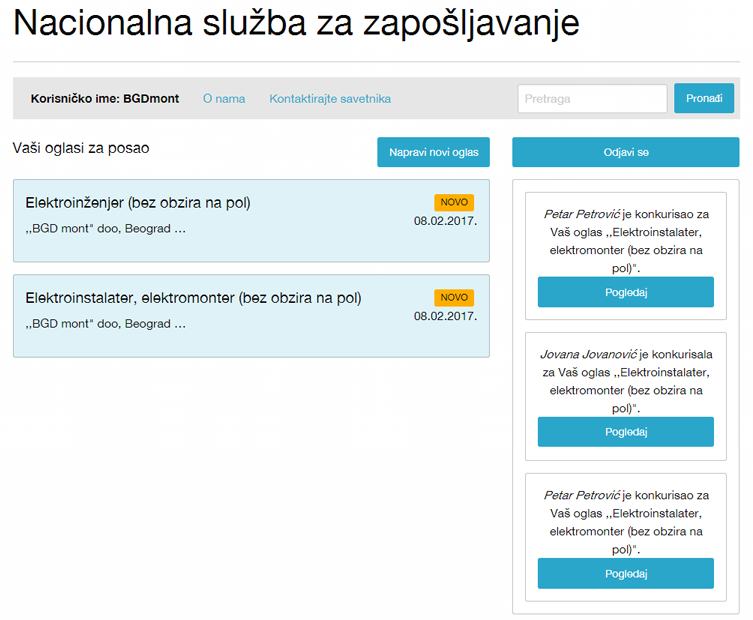
\includegraphics[width=\textwidth]{korisnicki-interfejs/slike/k-index.png}
	\caption{Kompanija: Po\v cetna strana.}
	\label{for: k-index}
\end{figure}

\begin{figure}[H]
	\centering
	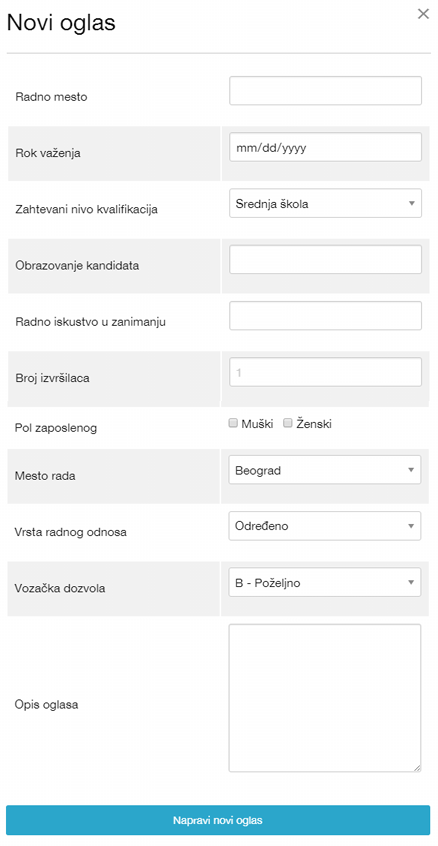
\includegraphics[height=0.95\textheight]{korisnicki-interfejs/slike/k-noviOglas.png}
	\caption{Kompanija: Novi oglas.}
	\label{for: k-noviOglas}
\end{figure}